\documentclass{beamer}
\usetheme{metropolis}           % Use metropolis theme
\usepackage[german]{babel}  
\usepackage[utf8]{inputenc}	%dt Sonderzeichen wie ß
\usepackage{tikz}
\usepackage{amssymb}
\usepackage{multirow}
\usepackage{pgfpages}
\usepackage{cite}
\usepackage{animate}

%\setbeameroption{show notes on second screen=right}  %% Uncomment this to get Notes
\usetikzlibrary{arrows,positioning}

\renewcommand*{\figurename}{Abb.}




\title{Efficient and Robust Automated Machine Learning}
\date{12. Juli 2018}
\author{Robert Feldhans}
\institute{Seminar Musterklassifikation}
\begin{document}
	\maketitle
	
	\begin{frame}{Inhalt}
		\setbeamertemplate{section in toc}[sections numbered]
		\tableofcontents[hideallsubsections]
	\end{frame}
	
	\section{Motivation}%%%%%%%%%%%%%%%%%%%%%%%%%%%%%%%%%%%%%%%%%%%%%%%%%%%%%%%%%%%%%%%%%%%%%
	
	\begin{frame}{Interlude: Hyperparameter I}
		Was sind Hyperparameter?
		\begin{itemize}
			\item Werden \emph{vor} dem Lernen definiert
			\item Sind in der Regel Zahlen oder Funktionen
		\end{itemize}
		\pause
		\begin{alertblock}{Allgemein}
			Alles was in irgendeiner Art austauschbar ist in einem speziellen ML-Verfahren und während des Trainings konstant bleibt
		\end{alertblock}
	\end{frame}
	
	\begin{frame}{Interlude: Hyperparameter II}
		Beispiele für Hyperparameter
		\begin{itemize}
			\item Lernrate
			\item Gewichte jeglicher Form
			\item Anzahl der Cluster in k-means clustering
			\item Aktivierungsfunktionen
			\item Anzahl der Hidden Layers in einem Netz
			\item Breite der Layers in einem Netz
		\end{itemize}
	\end{frame}
	
	\begin{frame}{Motivation}
		\begin{itemize}
			\item Ein gutes neuronales Netz zu trainieren ist schwer, braucht viel Arbeitszeit und Erfahrung
			\item Jeder sollte in der Lage sein NN zu trainieren (im besten Fall sogar Maschinen!)
		\end{itemize}
		\pause
		\alert{Lösung: Ein automatisches (und effizientes) System, welches gute Hyperparameter auswählt, muss her!}
	\end{frame}
	
	
	\section{Automated Machine Learning in a Nutshell}%%%%%%%%%%%%%%%%%%%%%%%%%%%%%%%%%%%%%%%%%%%%%%%%%%%%%%%%%%%%%%%%%%%%%%%%%%%%%%%%
	
	
	\begin{frame}{Auto-ML I}
		\begin{alertblock}{Grundlegende Idee}
			\begin{itemize}
				\item Starten mit \emph{irgendwie} ausgewählten Hyperparametern
				\item Classifier trainieren
				\item Classifier evaluieren
				\item Hyperparametertuning mithilfe eines Bayesian optimizer
				\item Wiederholung bis zu einem zufriedenstellenden Ergebnis
			\end{itemize}
		\end{alertblock}
	\end{frame}
	
	\begin{frame}{Auto-ML II}
		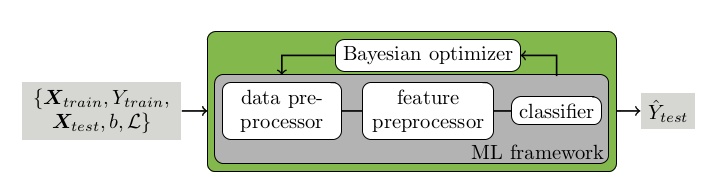
\includegraphics[width=\linewidth]{Bilder/MachineLeaningInANutshell}
	\end{frame}
	
	\begin{frame}{Initialisierung der Hyperparameter}
		Bild zu problemen mit der initialisierung von hyperparametern
	\end{frame}
	
	\begin{frame}{Rapidly Exploring Random Tree (RTT) I}
		\begin{alertblock}{Idee}
			\begin{itemize}
				\item Werte zufällig wählen
				\item So oft wiederholen, bis man einen guten Überblick über den Searchspace hat
			\end{itemize}
		\end{alertblock}
		\pause
		\begin{alertblock}{Vorteil}
			Bietet beliebig guten Überblick über den Searchspace
		\end{alertblock}
		\pause
		\begin{alertblock}{Achtung}
			RTT bietet einige Fallstricke. Think before use!
		\end{alertblock}
	\end{frame}
	
	\begin{frame}{Rapidly Exploring Random Tree (RTT) II}
		Gif coming as soon as i figured out animategraphics....
		%\animategraphics[autoplay,loop]{12}{RTT-}{0}{30}
	\end{frame}
	
	\begin{frame}{Probleme}
		\begin{itemize}
			\item Ausgesprochen Rechenintensiv
			\item Unterschiedliche Lernverfahren?
			\item Es gibt kein ``best'' Lernverfahren, nur ``best at''
			\item Manche ML-Verfahren erfordern intensive Hyperparameteroptimisierung
			\item Bayes optimization sollte sich jedoch um dieses Problem kümmern
		\end{itemize}
	\end{frame}
	
	\section{Meta Learning}%%%%%%%%%%%%%%%%%%%%%%%%%%%%%%%%%%%%%%%%%%%%%%%%%%%%%%%%%%%%%%%%%%%%%%%%%%%%%%%%
	
	
	
	\section{Ensembles}%%%%%%%%%%%%%%%%%%%%%%%%%%%%%%%%%%%%%%%%%%%%%%%%%%%%%%%%%%%%%%%%%%%%%%%%%%%%%%%%
	
	
	
	\begin{frame}{}
			Vielen Dank für eure Aufmerksamkeit!
	\end{frame}
	
	\section{Fragerunde}%%%%%%%%%%%%%%%%%%%%%%%%%%%%%%%%%%%%%%%%%%%%%%%%%%%%%%%%%%%%%%%%%%%%%%%%%%%%%%%%%%%%%%%%%
	
	\begin{frame}{Quellen}
		\bibliography{demo}
		\bibliographystyle{plain}
	\end{frame}
	
\end{document}
	
	
	